\chapter{De Methodo Orationis Mentalis Dom Vitalis Lehodey}
\begin{center}
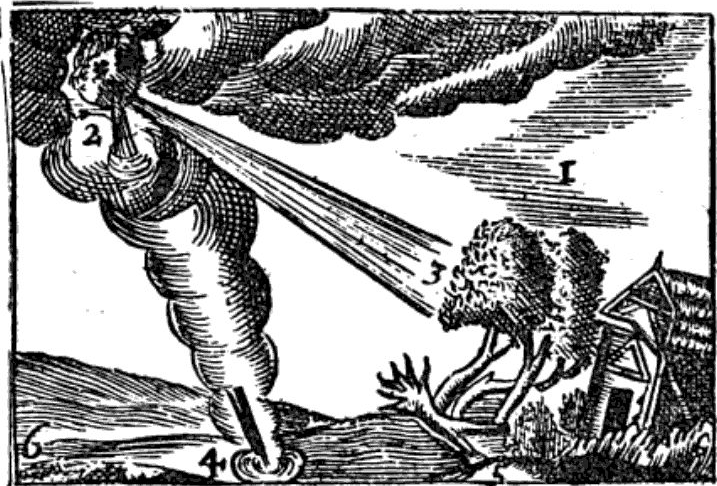
\includegraphics[scale=0.5]{Air.png}
\end{center}

\section{Intended Audience}
This is intended for students who have completed Lectio 7 and 8 of Latin by the Natural Method and Chapter 6 of Lingua Latina Per Se Illustrata. There are x words in this chapter.

Things to use:
	- Prope and Procul
	- Quam in comparison
	- Passive Verbs
	- Lots of Ablative
	- Locative Case 
	- Quo, Unde, Ubi
	- Fourth and Fifth Declension

\section{Text}
In silva Jeremias et Eliseus ambulaverunt. Jeremias dixit ad Eliseum "Unde venisti?". "Natus sum in Britannia, Ubi sumus?". "In Italia sumus. Non Romae, non Tusculi, non Tarentii, sed in Italia." Jeremias respondit. "Unde venisti?" interrogavit Eliseus. "Israel est ubi natus sum, ante Christum natum, sed natus es post Christum natum?". "Sum, duo milia anni post Christum natum.". Aura bona flat per arbores, et placet Jeremiae et Eliseo. "Bona aura est Silvae, flantur arbores.  Quo venit?" ait Eliseus. Respondit "Nescio. Deus scit, et scivit ante creationem mundi". "Sicut Deus spirat super nos.  Bene flat haec aura. Ignis non tam bonus est quam aura." ait Eliseus. "Quid? non placet tibi ignis meus? Aura tam bona non est quam ignis. Haec frigida aura non tam calida est quam ignis." respondit Jeremias. "Vetus vir!" exclamavit Eliseus "Senectus tuus cepit laetitiam bonae aurae ex te". "Cepit" respondit "Noli exclamare de hac re". "Sed" Jeremias addidit "non cepit Ventus Dei, flat in corde meo". 

"Quid est hic ventus?" interrogavit Eliseus. "Ventus, vel ignis orationis meae qui spirat in me". "Ignis? Quid ignis". "Ignis orationis mentalis" respondit "Qui instruxit me in amore et virtute, Ventus cognitionis Dei, non sicut scientia theologiae". "Quomodo habeo cognitionem Dei? Volo habere procellam Cognitionis Dei.". "Procella? Cur interrogavisti rem parvam? Cur non interrogavisti turbinem? Deus apparuit Moysi in Aegypto, et fuit in turbine flammae. Haec turbo duxit populum eius ex Aegypto. Cur procellam solam interrogavisti? Deus amat eum qui vult meliorem amorem.". "Quomodo facio orationem mentalem?" interrogavit. 

"Dicebam de methodo Dom Vitalis Lehoedy. Scripsit librum." respondit Jeremias. "Primo, Franciscus Salensius Sanctus dixit facere unam horam orationis mentali in die una. Lehodey (qui scripsit vias orationis mentalis (Ways of Mental Prayer anglice), quem auscultas, dixit facere dimidiam partem horae. Potes loqui cum presbytero de tempore orationis mentalis. ". "Deinde?" respondit Eliseus". "Tolle librum, qui est de vitiis, vel de virtutibus, vel de mysteriis Fidei. Quicumque bonus est tibi. Liber quem Lehodey dixit bonum appelatur "Preparation For Death" vel praeparatio mortis, quae scriptus est a Sancto Alphonso a Ligorio". "Deinde" perrexit Jeremias "Tolle paginam, et legi eam quater. Fac hanc rem quia in mente debeo habere paginam.". "Sicut dixit David in Psalmo Primo, "Beatus vir qui meditabitur in lege sua die ac nocte."" dixit Eliseus. "Bene dixisti, Elisee, in hoc modo meditari possumus". "Deinde, cogita de hac re in paginam est. Fortasse, de patientia Christi in cruce, vel de lege nova. Cogita "Quomodo possum facere praecepta Domini?" vel "Quomodo possum diligere Deum sicut is diligit me?". "Intellego" respondit Eliseus. "Deinde, ex consideratione hac, ora ad Deum. Consideratio non est oratio, sed consideratio dat auxilium orationi. Dice Deo de consideratione, in precibus interroga gratias ex eo. Postremo, fac resolutionem ex precibus et ex consideratione. Dici Deum "Fecero hanc rem, quam facere necesse est.". 

Subito, Procella flat, et arbores sternebantur. Procella sternebat arbores. Foenum etiam sternebantur a procella. . Arbor cedidit inter Jeremiam et Eliseum. Ceciderunt in terra. "Bene valesne?" Eliseus interrogavit. "Valeo" respondit Jeremias.  Deinde, terra movet se. "Quid, iam terraemotus?". "In temporibus antiquis, cogitaverunt quod Terraemotus accidit quia venti subterranei flant, et terra movetur a his ventis. Jeremias surrexit et stravit manum suam "Veni mecum". Jeremias cepit manum Elisei et traxit eam. Eliseus stavit, deinde ambulaverunt in Silvam.

   

\footnote{\textbf{ūrēbat} = It was burning}